\documentclass[11pt]{article}
\usepackage[margin=2.3cm]{geometry}
\usepackage{amsmath,amssymb}
\usepackage{booktabs}
\usepackage{graphicx}
\usepackage[hidelinks]{hyperref}
\usepackage{microtype}

\title{Particle Gibbs BART with the one-step optimal proposal}
\author{Branch \texttt{pgbart}, short report}
\date{27 November 2026}

\begin{document}
\maketitle

\section{Summary}

Particle Gibbs (PG) replaces the local tree moves of BART by a conditional SMC run that proposes a whole tree.
Our PG implementation used the bootstrap proposal of Lakshminarayanan, Roy, and Teh (2015), which draws each node decision from the prior.
We added the one-step optimal proposal of their 2013 paper, which draws each decision from its conditional given the data.
We call the new sampler PG-opt.
We ran it on Abalone, SeoulBike, and Friedman with the paper's protocol: 5 runs, 4 chains, $10^4$ iterations, 100 trees, $C=10$ particles.
On Abalone, PG-opt mixes better than every method in the paper.
On Friedman, it mixes as well as MTMH+PT.
On SeoulBike, its noise variance comes closest to the long Default run, but its chains still disagree.
It costs 9 to 16 times Default per iteration.

\section{Method}

A tree is built top-down in breadth-first order.
At a node of depth $d$ with training rows $I$, the prior splits with probability $p_d = \alpha(1+d)^{-\beta}$, picks variable $v$ with probability $s_v$, and picks a threshold uniformly from the grid $G_v$.
Let $\ell(I)$ be the collapsed log marginal likelihood of a leaf holding $I$.
The optimal proposal draws the decision from the masses
\begin{align*}
  w_{\text{stop}} &= 1 - p_d, \\
  w_{v,\tau} &= p_d \, \frac{s_v}{|G_v|} \, \exp\bigl\{\ell(I_L) + \ell(I_R) - \ell(I)\bigr\},
\end{align*}
with $w_{v,\tau}=0$ when a child would be empty.
The particle weight is multiplied by the normaliser $Z = w_{\text{stop}} + \sum_{v,\tau} w_{v,\tau}$.
$Z$ depends on the node only, so the reference particle that replays the old tree receives the same factor.
The bootstrap proposal instead draws from the prior and multiplies the weight by the likelihood ratio of the split drawn.
Both proposals target the same truncated prior as the Default sampler, so all chains share one posterior.
Resampling is multinomial after every stage, and the output tree is drawn from the final weights.

\section{Implementation}

The code is on branch \texttt{pgbart} of \texttt{yanshuotan/bart-playground}.
\begin{itemize}
  \item \texttt{bart\_playground/pg\_kernels.py}: the conditional SMC kernel in Numba, for both proposals.
  \item \texttt{PGBART(proposal="optimal" | "prior")} in \texttt{bart.py} and \texttt{PGSampler} in \texttt{samplers.py}; the default is \texttt{"optimal"}.
  \item \texttt{diagnosis/run\_fixed100.py}: method names \texttt{pg} (bootstrap) and \texttt{pg\_opt}.
  \item \texttt{diagnosis/pg/compare\_pg\_opt.py}: the tables and figure of this report.
\end{itemize}
Each covariate is binned once against its threshold grid.
Row $i$ goes left of the $j$-th threshold of $v$ exactly when its bin index is at most $j$.
One pass over a node's rows then fills the count and residual-sum histograms of every variable.
Cumulative sums of these histograms give the likelihood ratio of every split, so $Z$ costs $O(|I|\,p + \sum_v |G_v|)$ per node.
$Z$ and the per-variable masses are cached on the node, and drawing the threshold needs one more pass over the chosen variable.
Particles share nodes, and particles that make the same split of a shared node also share its children.
Repeated thresholds, which quantile grids of discrete columns produce, keep their prior share and give the same partition.

Three checks support correctness.
A unit test enumerates every tree of a small problem and matches the PG draws to the exact posterior, for both proposals and for a grid with a repeated threshold.
A second test matches the cached split masses to direct enumeration.
The bootstrap path gives bit-identical draws before and after the change.

\section{Results}

Each PG run refitted Default in the same job, and cost is PG fit time over that Default's.
These Default draws equal the paper store's in all 15 runs.
The paper methods come from the paper store.
Table~\ref{tab:main} uses the last 7000 draws of each chain.

\begin{table}[ht]
\centering
\small
\begin{tabular}{llcccccc}
\toprule
 & & Default & Default+PT & MTMH & MTMH+PT & PG & PG-opt \\
\midrule
Abalone & $\hat R$ median & 1.097 & 1.029 & 1.031 & 1.013 & 1.034 & \textbf{1.005} \\
 & $\hat R$ 90\% & 1.248 & 1.071 & 1.087 & 1.035 & 1.092 & \textbf{1.016} \\
 & between/within & 0.139 & 0.046 & 0.048 & 0.016 & 0.052 & \textbf{0.007} \\
 & test RMSE & 1.976 & 1.964 & 1.956 & 1.956 & 1.966 & 1.954 \\
 & cost / Default & 1 & & & & 3.9 & 9.6 \\
\midrule
SeoulBike & $\hat R$ median & 1.466 & \textbf{1.220} & 1.415 & 1.278 & 1.412 & 1.377 \\
 & $\hat R$ 90\% & 1.913 & \textbf{1.462} & 1.842 & 1.570 & 1.896 & 1.857 \\
 & between/within & 1.10 & \textbf{0.37} & 1.20 & 0.68 & 1.35 & 1.57 \\
 & test RMSE & 233.5 & 233.1 & 245.2 & 248.0 & 248.2 & 267.4 \\
 & cost / Default & 1 & & & & 4.6 & 16.0 \\
\midrule
Friedman & $\hat R$ median & 1.233 & 1.052 & 1.108 & 1.028 & 1.108 & \textbf{1.026} \\
 & $\hat R$ 90\% & 1.482 & 1.100 & 1.254 & \textbf{1.058} & 1.231 & 1.065 \\
 & between/within & 0.345 & 0.061 & 0.146 & \textbf{0.032} & 0.162 & 0.033 \\
 & test RMSE & 1.143 & 1.120 & 1.141 & 1.128 & 1.134 & 1.132 \\
 & cost / Default & 1 & & & & 3.3 & 9.2 \\
\bottomrule
\end{tabular}
\caption{Means over 5 runs. $\hat R$ is the rank-normalised split $\hat R$ of the 100 test predictions. Between/within is the ratio of between-chain to within-chain spread of the prediction vector. Cost is fit time per chain relative to Default.}
\label{tab:main}
\end{table}

\paragraph{Abalone.}
PG-opt has the lowest $\hat R$ and the lowest between/within ratio of all six methods.
Its between/within ratio is one seventh of bootstrap PG's and less than half of MTMH+PT's.
Its $\sigma^2$ trace reaches the long Default band within about 10 iterations (Figure~\ref{fig:sigma}).
It changes 46 of 100 trees per iteration, against 28 for bootstrap PG.

\paragraph{SeoulBike.}
After burn-in, the mean $\sigma^2$ is $1.5\times10^{-3}$ for the long Default run, $3.0\times10^{-3}$ for Default, $2.8\times10^{-3}$ for PG, and $1.8\times10^{-3}$ for PG-opt.
PG-opt has therefore moved much further toward the posterior than any other short-chain method.
Its test RMSE moves the same way: the long Default run gives 258.7 on these test sets, above every short chain except PG-opt.
The chains still disagree, so $\hat R$ stays high for every method.
PG-opt changes 31 of 100 trees per iteration, against 13 for bootstrap PG.

\paragraph{Friedman.}
PG-opt and MTMH+PT have the lowest $\hat R$ and between/within ratio, about one fifth of bootstrap PG's.
PG-opt changes 44 of 100 trees per iteration, against 24 for bootstrap PG.

\begin{figure}[ht]
\centering
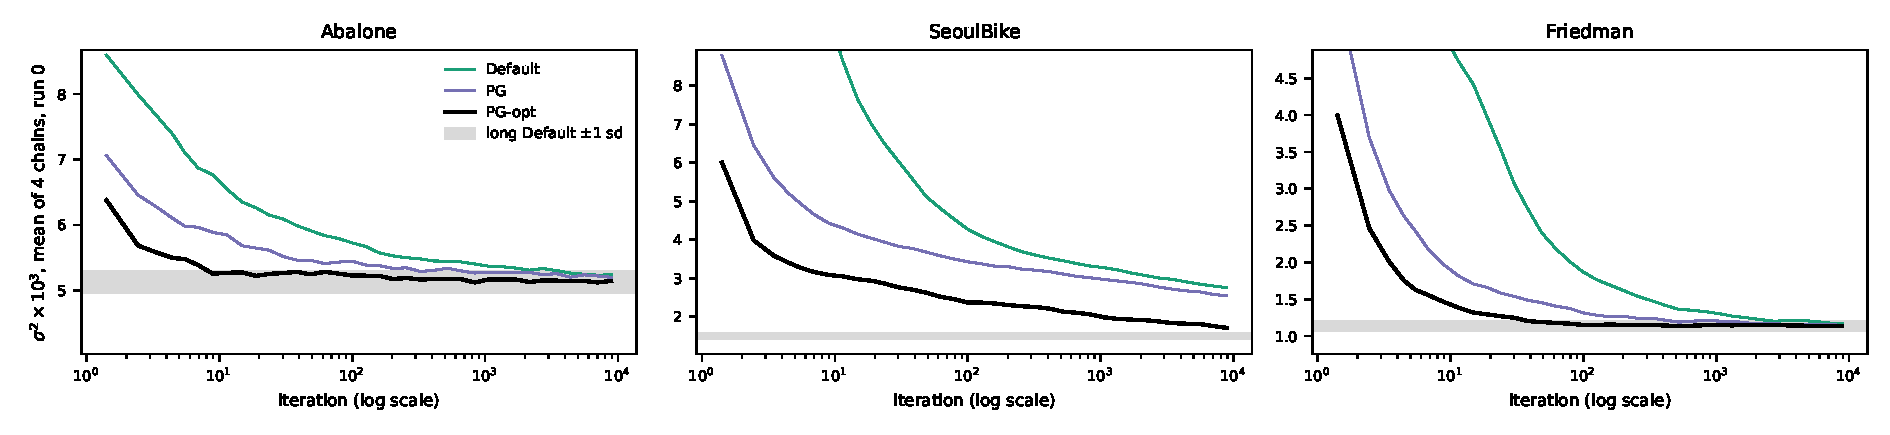
\includegraphics[width=\linewidth]{pg_opt_sigma2.pdf}
\caption{Noise variance $\sigma^2$ against iteration, run 0, mean of 4 chains, binned on a log scale. The grey band is the long Default run's mean $\pm 1$ sd.}
\label{fig:sigma}
\end{figure}

\section{Hypercube check}

On the Hypercube-$D$ problems of the PG paper, PG-opt reaches a higher training log-likelihood than bootstrap PG on both grids (mean of 5 seeds, last 1000 of 2000 iterations).
On the uniform grid the values for $D = 3, 4, 5, 7$ are 190, 199, 244, and 438 for PG-opt, against 152, 157, 174, and 378 for PG.
CGM (Default) still reaches 233, 512, 523, and 669.
On the quantile grid PG-opt exceeds CGM at $D = 4$ and $D = 7$.

\section{Adaptive resampling}

Resampling after every stage lets a small tree take over.
A finished particle keeps its weight, while an unfinished one is multiplied by some $Z<1$ at each stage.
On the $D=7$ uniform Hypercube, two of five PG-opt chains stayed at one leaf for all 2000 iterations.
The 2013 paper resamples only when the effective sample size falls below a fraction of $C$.
We tried this with thresholds $0.1\,C$ (with $C=10$, no resampling at all) and $0.5\,C$.
Both fixed the Hypercube failure, with log-likelihoods of 1653 and 829 at $D=7$, against 669 for CGM.
On the three datasets neither improved mixing.
The between/within ratio went from 1.57 to 1.99 and 1.69 on SeoulBike, from 0.007 to 0.009 and 0.008 on Abalone, and from 0.033 to 0.043 and 0.028 on Friedman.
Cost rose to 13 to 25 times Default.
We therefore kept resampling after every stage.

\end{document}
